The cross section of $Z$ boson production in association with heavy flavour ($b,c$) jets is known to be not well predicted by the Sherpa MC and so these processes are normalised to data in a control region. Since the production of jets is independent of the decay mode of the $Z$ boson, $Z \rightarrow \mu\mu/ee$ + heavy flavour jets are selected as this provides a high purity sample that is orthogonal to the signal regions selection and can be included in the final fit to determine the Z+HF normalisation from data.

The events falling in the control region are selected as follows:

\begin{itemize}
\item Events selected with $bbll$ trigger selection~\cite{Olsson:2765838} using single-lepton and di-lepton triggers (reported in Figure~\ref{fig:bbllTriggers});
\item Exactly two muons or two electrons with opposite-sign charges;
\item Exactly two $b$-tagged jets (using DL1r 77\% working point);
\item 75 GeV $<m_{ll}<$ 110 GeV (select Z mass peak);
\item $m_{bb}<$40 GeV or $m_{bb}>$210 GeV (to veto Higgs mass peak and to ensure orthogonality to $bb\ell\ell$ signal region).
\end{itemize}

\begin{figure}
\centering
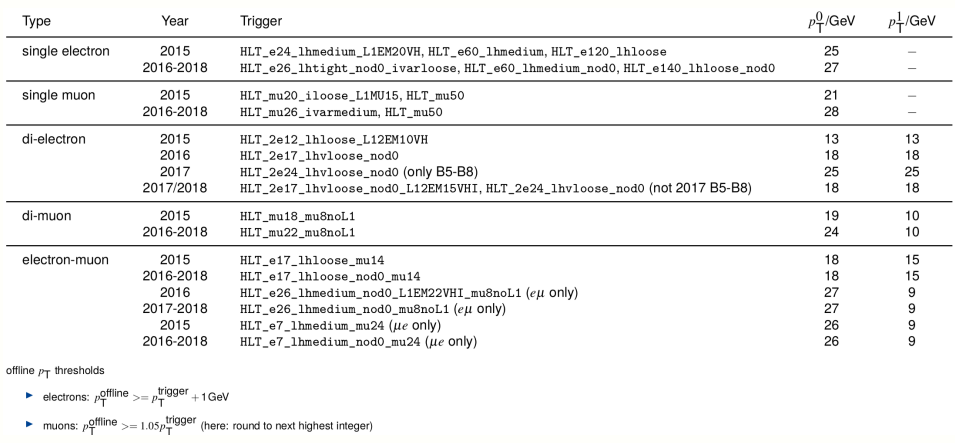
\includegraphics[width=.9\textwidth]{figures/selection/bbllTriggers}
\caption{Triggers used for data-taking for the Z+HF control regions events (from the $bb\ell\ell$ analysis).}
\label{fig:bbllTriggers}
\end{figure}

This selection has been harmonised with the selection of the $Z+$HF control region applied in the di-Higgs to $bbll$ analysis in order to use the same definition of the control region and simplify its inclusion in the di-Higgs combination (the control region used in this $bb\tau\tau$ analysis is built using the $bbll$ analysis framework and it is common for the two analyses). 

This region is dominated by $Z+$HF events followed by $t\bar{t}$ events as shown in Table~\ref{tab:Yields_ZHF_prefit} reporting the event yields for the processes entering the $Z+$HF control region. 

\begin{table}[h]
  \centering
  \begin{tabular}{lll}
  \hline
  \hline
Process & Yields\\ 
$Z \rightarrow ee$ & 20132.2507877 $\pm$ 163.697540715\\
$Z \rightarrow \mu\mu$ & 26718.1411476 $\pm$ 225.441215886\\
$t\bar{t}$ & 34909.8856201 $\pm$ 39.0175844078\\
Total background &  83464.0578613 $\pm$ 281.699638149 \\
Data & 96032\\
\hline
\hline
\end{tabular}
 \caption{Pre-fit event yields in the Z+HF control region.}
  \label{tab:Yields_ZHF_prefit}
\end{table}


This control region is included in the final fit as $m_{ll}$ distribution shown in Figure~\ref{fig:mll_ZHF_prefit}. Given the large fraction of \ttbar events and the high purity for this background in the tails of the $m_{ll}$ distribution, this region has good constraining power not only on Z+hf but also on \ttbar.

From a fit to data of this CR alone, shown in Appendix~\ref{subsec:appendix_fit_ZCR}, the normalisation of the Z+HF background is found to be $1.38 \pm 0.11$ (expected and in agreement with normalisation found also in other analyses) and the normalisation of the \ttbar background is found to be $0.97 \pm 0.04$.

\begin{figure}
\centering
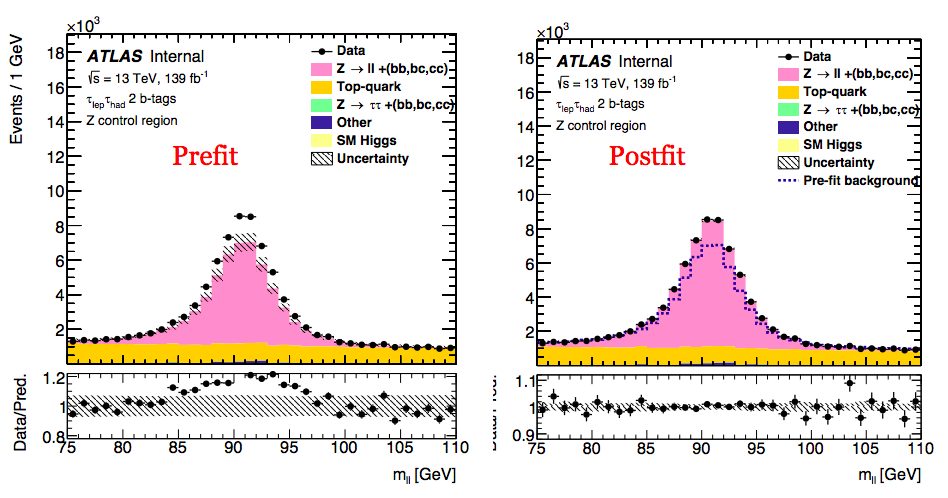
\includegraphics[width=.9\textwidth]{figures/selection/ZHF_mll}
\caption{Pre-fit and post-fit $m_{ll}$ distribution in the Z+HF control region. Note: plot done with an older version of inputs with \ttbar reweighting included, which result in slightly higher \ttbar normalisation factor of $0.99 \pm 0.04$.}
\label{fig:mll_ZHF_prefit}
\end{figure}

Additional studies on the definition of the CR are reported in Appendix~\ref{subsec:appendix_selection_ZHFCR}.
